% Foucault's experiment to measure the speed of light (1862)

\documentclass[tikz, border = 1 cm]{standalone}

\usepackage{tikz}
\usetikzlibrary{optics}

\begin{document}
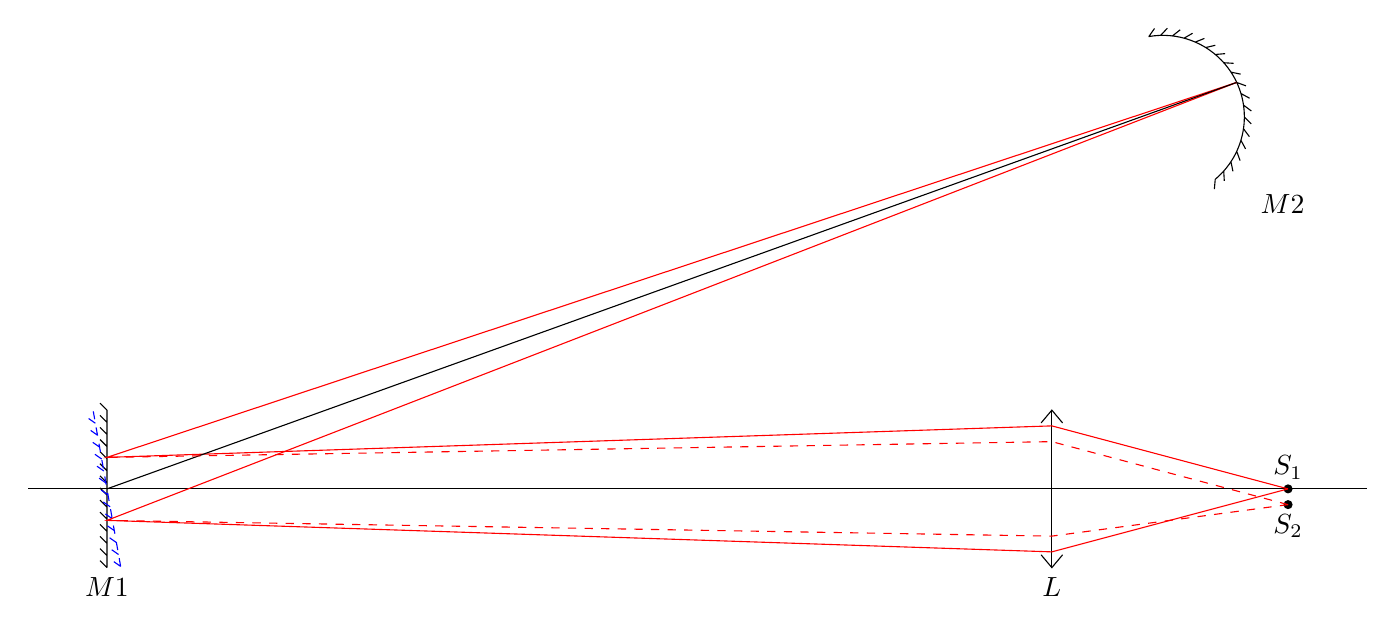
\begin{tikzpicture}[use optics]
 \draw (6,0) -- (-11,0);
 \filldraw (5,0) circle (0.05);
  \node[above] at (5,0) {$S_1$};
 
 \filldraw (5,-.2) circle (0.05);
 \node[below] at (5,-.2) {$S_2$};
 \node[lens,label={[align=center]below:$L$}] at (2,0) (L) {};
 \node[mirror,rotate=180,label={[align=center]above:$M1$}] (M1) at (-10,0) {};
 \node[mirror,dashed,blue,rotate=190] (M1prime) at (-10,0) {};
 
 \node[concave mirror,rotate=25, label={[label distance=0.25cm]south:$M2$}] at (4cm,5) (M2) {};

 \draw[red] (5,0) -- (L.lens north) -- (-10,0.4) -- (M2.arc center);
 \draw[red] (5,0) -- (L.lens south) -- (-10,-0.4) -- (M2.arc center);

 \draw (M1.center) -- (M2.arc center);
 
 \draw[red,dashed] (5,-0.2) -- (2,0.6) -- (-10,0.4);
 \draw[red,dashed] (5,-0.2) -- (2,-0.6) -- (-10,-0.4);

\end{tikzpicture}
\end{document}
